\documentclass[10pt, export]{beamer}

\usepackage[utf8]{inputenc}
\usepackage[T1]{fontenc}

\usepackage{standalone}
    
\usepackage[acronym]{glossaries}
    
\usepackage{enumitem}
    
\usepackage{multirow}
\usepackage{multicol}
    
\usepackage{array}
\newcolumntype{x}[1]{>{\centering\let\newline\\\arraybackslash\hspace{0pt}}p{#1}}
\usepackage{booktabs, colortbl}
    
\usepackage{siunitx}
\usepackage{mathrsfs, amsmath}

\usepackage{graphicx}
\usepackage{subcaption}
\usepackage[font={small, color=IGNDarkGrey}, labelformat=empty]{caption}
\DeclareCaptionFont{footnotesize}{\footnotesize}
\usepackage[font={footnotesize, color=IGNDarkGrey}, labelformat=empty]{subcaption}
\usepackage{adjustbox}

\usepackage{tikz}
\usetikzlibrary{calc, 3d, shapes, arrows, shadows, decorations}

\usepackage{pgfplots, pgfplotstable}


\usepackage{pifont, textcomp}
\newcommand{\cmark}{{\color{green} \ding{51}}}%
\newcommand{\xmark}{{\color{red} \ding{55}}}%

\definecolor{Moins4}{RGB}{183,10,10}
\definecolor{Moins3}{RGB}{255,0,0}
\definecolor{Moins2}{RGB}{255,122,12}
\definecolor{Moins1}{RGB}{255,181,12}
\definecolor{Zero}{RGB}{255,255,255}
\definecolor{Plus1}{RGB}{58,255,12}
\definecolor{Plus2}{RGB}{58,155,12}


\usepackage{hyperref}

\usepackage[useregional]{datetime2}
    
\usepackage[
        backend=biber,
        style=alphabetic,
        backref=true,
        sorting=none,
        autocite=footnote,
        maxnames=2,
        hyperref=true,
        natbib=false,
        abbreviate=false,
        doi=false,
        isbn=false,
        url=false
    ]{biblatex}
\addbibresource{references.bib}
\setbeamerfont{footnote}{size=\tiny}


\usetheme{ign}


\newacronym{acr::lod}{LoD}{Level of Detail}
\newacronym{acr::elod}{eLoD}{evaluation Level of Detail}
\newacronym{acr::lidar}{LiDAR}{Light Detection and Ranging}
\newacronym{acr::dsm}{DSM}{Digital Surface Model}
\newacronym{acr::gui}{GUI}{Graphical User Interface}

\title{The necessary yet complex evaluation of 3D city models}
\subtitle{a semantic approach}
\date{\tiny \DTMdisplaydate{2019}{5}{23}{4}}
\author{
    \scriptsize \underline{\textbf{Oussama Ennafii}} \inst{1, 2}, Arnaud Le Bris \inst{1}, Cl\'ement Mallet \inst{1}, Florent Lafarge \inst{2}
}
\institute{
    \scriptsize \inst{1} Univ. Paris Est, LaSTIG STRUDEL, IGN, ENSG\\
    \inst{1} name.surname@ign.fr\\
    ~\\
    \scriptsize \inst{2} Inria, TITANE\\
    \inst{2} name.surname@inria.fr
}

\addtocounter{framenumber}{20}

\begin{document}
    \begin{frame}{3D representation of buildings}
        \begin{figure}
            \begin{center}
                \includestandalone[mode=buildnew, width=.9\textwidth]{building_models-all}
            \end{center}
        \end{figure}
    \end{frame}
    \begin{frame}{Naming convention: 3D model vs. 3D mesh}
        \begin{figure}
            \begin{center}
                \begin{subfigure}{\textwidth}
                    \begin{center}
                        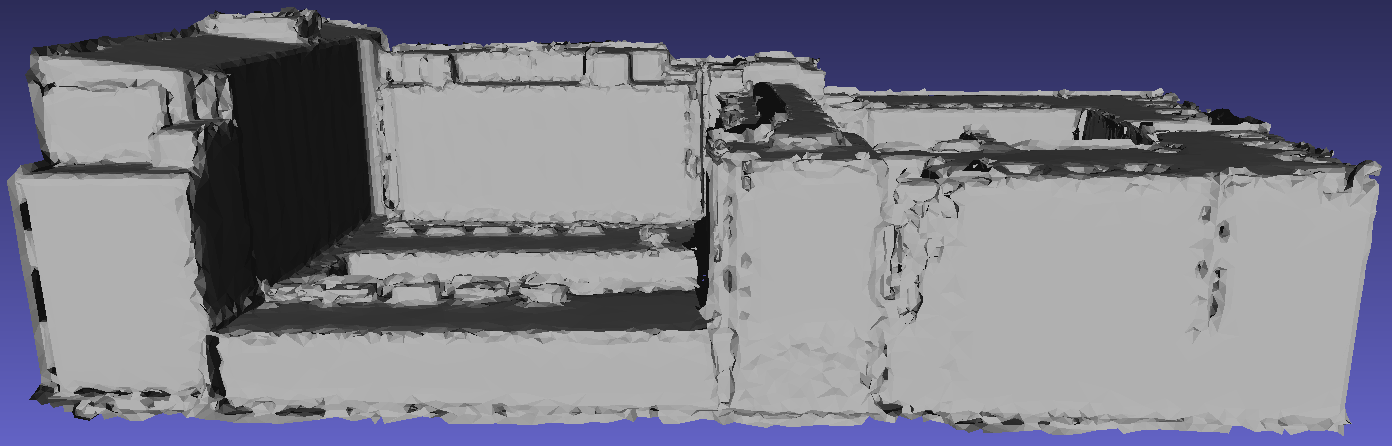
\includegraphics[height=.28\textheight]{images/difference_mesh_model/bercy_building_mesh_1_e5}
                        \caption{\underline{3D mesh} of a building surface ($\approx$ \num[output-exponent-marker = \text{e}]{1e5} triangles).}
                    \end{center}
                \end{subfigure}
                \\
                \begin{subfigure}{\textwidth}
                    \begin{center}
                        \includestandalone[mode=buildnew, height=.28\textheight]{ground_truth_model}
                        \caption{Building \underline{3D polyhedral model} ($\approx$ 800 facets).}
                    \end{center}
                \end{subfigure}
                \caption{Different model schemes of a building ($\approx$ \SI{139 x 71 x 23}{\metre}).}
            \end{center}
        \end{figure}
    \end{frame}
    \begin{frame}{Geometric features}
        \begin{figure}
            \includestandalone[mode=buildnew, height=.62\textheight]{geometric_features}
        \end{figure}
        \begin{itemize}[label=$\blacktriangleright$, font=\color{IGNGreen}]
            \item \footnotesize Statistics are computed, for each \underline{attribute}, at \underline{building} level.
            \item \footnotesize Results are concatenated in a \underline{fixed size} feature vector (\textit{length = 20} in experiments).
        \end{itemize}
    \end{frame}
    \begin{frame}{Height-based features}
        \begin{figure}
            \includestandalone[mode=buildnew, width=\textwidth]{altimetric_features}
        \end{figure}
        \begin{itemize}[label=$\blacktriangleright$, font=\color{IGNGreen}]
            \item \footnotesize Feature vectors consist on the concatenated histogram values.
            \item \footnotesize The histogram resolution is \underline{constant} (\textit{length = 20} in experiments).
        \end{itemize}
    \end{frame}
    \begin{frame}{Image-based features}
        \begin{figure}
            \begin{center}
                \includestandalone[mode=buildnew, width=.9\textwidth]{radiometric_features}
            \end{center}
        \end{figure}
        \begin{itemize}[label=$\blacktriangleright$, font=\color{IGNGreen}]
            \item \footnotesize A \underline{histogram} of the cosine similarity is computed \underline{per edge}.
            \item \footnotesize A \underline{weighted sum} of all edge histograms is computed \underline{over the building}.
            \item \footnotesize All histograms having the same resolution result in a feature vector (\textit{length = 20} in experiments).
        \end{itemize}
    \end{frame}
    \begin{frame}{Datasets: errors occurences}
        \only<1>{
            \begin{figure}
                \begin{center}
                    \includestandalone[mode=buildmissing, width=.7\textwidth]{dataset_stats_building}
                \end{center}
            \end{figure}
        }
        \only<2->{
            \begin{figure}
                \begin{center}
                    \includestandalone[mode=buildmissing, width=.8\textwidth]{dataset_stats_facet}
                \end{center}
            \end{figure}
        }
    \end{frame}
    \begin{frame}{Feature importance}
        \only<1>{
            \begin{figure}
                \includestandalone[mode=buildnew, width=.846\textwidth]{feat_imp_building}
            \end{figure}
        }
        \only<2->{
            \begin{figure}
                \includestandalone[mode=buildnew, width=\textwidth]{feat_imp_facet}
            \end{figure}
        }
    \end{frame}
\end{document}